\documentclass{beamer}
\usepackage[utf8]{inputenc}
\usepackage{fontawesome}
\usepackage{hyperref}

\usepackage{utopia} %font utopia imported
% \setbeamercovered{transparent}

\usetheme{Warsaw}
%%%%% NEW MATH DEFINITIONS %%%%%
\usepackage{bm}
% Mark sections of captions for referring to divisions of figures
\newcommand{\figleft}{{\em (Left)}}
\newcommand{\figcenter}{{\em (Center)}}
\newcommand{\figright}{{\em (Right)}}
\newcommand{\figtop}{{\em (Top)}}
\newcommand{\figbottom}{{\em (Bottom)}}
\newcommand{\captiona}{{\em (a)}}
\newcommand{\captionb}{{\em (b)}}
\newcommand{\captionc}{{\em (c)}}
\newcommand{\captiond}{{\em (d)}}

% Highlight a newly defined term
\newcommand{\newterm}[1]{{\bf #1}}


% Figure reference, lower-case.
\def\figref#1{figure~\ref{#1}}
% Figure reference, capital. For start of sentence
\def\Figref#1{Figure~\ref{#1}}
\def\twofigref#1#2{figures \ref{#1} and \ref{#2}}
\def\quadfigref#1#2#3#4{figures \ref{#1}, \ref{#2}, \ref{#3} and \ref{#4}}
% Section reference, lower-case.
\def\secref#1{section~\ref{#1}}
% Section reference, capital.
\def\Secref#1{Section~\ref{#1}}
% Reference to two sections.
\def\twosecrefs#1#2{sections \ref{#1} and \ref{#2}}
% Reference to three sections.
\def\secrefs#1#2#3{sections \ref{#1}, \ref{#2} and \ref{#3}}
% Reference to an equation, lower-case.
\def\eqref#1{equation~\ref{#1}}
% Reference to an equation, upper case
\def\Eqref#1{Equation~\ref{#1}}
% A raw reference to an equation---avoid using if possible
\def\plaineqref#1{\ref{#1}}
% Reference to a chapter, lower-case.
\def\chapref#1{chapter~\ref{#1}}
% Reference to an equation, upper case.
\def\Chapref#1{Chapter~\ref{#1}}
% Reference to a range of chapters
\def\rangechapref#1#2{chapters\ref{#1}--\ref{#2}}
% Reference to an algorithm, lower-case.
\def\algref#1{algorithm~\ref{#1}}
% Reference to an algorithm, upper case.
\def\Algref#1{Algorithm~\ref{#1}}
\def\twoalgref#1#2{algorithms \ref{#1} and \ref{#2}}
\def\Twoalgref#1#2{Algorithms \ref{#1} and \ref{#2}}
% Reference to a part, lower case
\def\partref#1{part~\ref{#1}}
% Reference to a part, upper case
\def\Partref#1{Part~\ref{#1}}
\def\twopartref#1#2{parts \ref{#1} and \ref{#2}}

\def\ceil#1{\lceil #1 \rceil}
\def\floor#1{\lfloor #1 \rfloor}
\def\1{\bm{1}}
\newcommand{\train}{\mathcal{D}}
\newcommand{\valid}{\mathcal{D_{\mathrm{valid}}}}
\newcommand{\test}{\mathcal{D_{\mathrm{test}}}}

\def\eps{{\epsilon}}


% Random variables
\def\reta{{\textnormal{$\eta$}}}
\def\ra{{\textnormal{a}}}
\def\rb{{\textnormal{b}}}
\def\rc{{\textnormal{c}}}
\def\rd{{\textnormal{d}}}
\def\re{{\textnormal{e}}}
\def\rf{{\textnormal{f}}}
\def\rg{{\textnormal{g}}}
\def\rh{{\textnormal{h}}}
\def\ri{{\textnormal{i}}}
\def\rj{{\textnormal{j}}}
\def\rk{{\textnormal{k}}}
\def\rl{{\textnormal{l}}}
% rm is already a command, just don't name any random variables m
\def\rn{{\textnormal{n}}}
\def\ro{{\textnormal{o}}}
\def\rp{{\textnormal{p}}}
\def\rq{{\textnormal{q}}}
\def\rr{{\textnormal{r}}}
\def\rs{{\textnormal{s}}}
\def\rt{{\textnormal{t}}}
\def\ru{{\textnormal{u}}}
\def\rv{{\textnormal{v}}}
\def\rw{{\textnormal{w}}}
\def\rx{{\textnormal{x}}}
\def\ry{{\textnormal{y}}}
\def\rz{{\textnormal{z}}}

% Random vectors
\def\rvepsilon{{\mathbf{\epsilon}}}
\def\rvtheta{{\mathbf{\theta}}}
\def\rva{{\mathbf{a}}}
\def\rvb{{\mathbf{b}}}
\def\rvc{{\mathbf{c}}}
\def\rvd{{\mathbf{d}}}
\def\rve{{\mathbf{e}}}
\def\rvf{{\mathbf{f}}}
\def\rvg{{\mathbf{g}}}
\def\rvh{{\mathbf{h}}}
\def\rvu{{\mathbf{i}}}
\def\rvj{{\mathbf{j}}}
\def\rvk{{\mathbf{k}}}
\def\rvl{{\mathbf{l}}}
\def\rvm{{\mathbf{m}}}
\def\rvn{{\mathbf{n}}}
\def\rvo{{\mathbf{o}}}
\def\rvp{{\mathbf{p}}}
\def\rvq{{\mathbf{q}}}
\def\rvr{{\mathbf{r}}}
\def\rvs{{\mathbf{s}}}
\def\rvt{{\mathbf{t}}}
\def\rvu{{\mathbf{u}}}
\def\rvv{{\mathbf{v}}}
\def\rvw{{\mathbf{w}}}
\def\rvx{{\mathbf{x}}}
\def\rvy{{\mathbf{y}}}
\def\rvz{{\mathbf{z}}}

% Elements of random vectors
\def\erva{{\textnormal{a}}}
\def\ervb{{\textnormal{b}}}
\def\ervc{{\textnormal{c}}}
\def\ervd{{\textnormal{d}}}
\def\erve{{\textnormal{e}}}
\def\ervf{{\textnormal{f}}}
\def\ervg{{\textnormal{g}}}
\def\ervh{{\textnormal{h}}}
\def\ervi{{\textnormal{i}}}
\def\ervj{{\textnormal{j}}}
\def\ervk{{\textnormal{k}}}
\def\ervl{{\textnormal{l}}}
\def\ervm{{\textnormal{m}}}
\def\ervn{{\textnormal{n}}}
\def\ervo{{\textnormal{o}}}
\def\ervp{{\textnormal{p}}}
\def\ervq{{\textnormal{q}}}
\def\ervr{{\textnormal{r}}}
\def\ervs{{\textnormal{s}}}
\def\ervt{{\textnormal{t}}}
\def\ervu{{\textnormal{u}}}
\def\ervv{{\textnormal{v}}}
\def\ervw{{\textnormal{w}}}
\def\ervx{{\textnormal{x}}}
\def\ervy{{\textnormal{y}}}
\def\ervz{{\textnormal{z}}}

% Random matrices
\def\rmA{{\mathbf{A}}}
\def\rmB{{\mathbf{B}}}
\def\rmC{{\mathbf{C}}}
\def\rmD{{\mathbf{D}}}
\def\rmE{{\mathbf{E}}}
\def\rmF{{\mathbf{F}}}
\def\rmG{{\mathbf{G}}}
\def\rmH{{\mathbf{H}}}
\def\rmI{{\mathbf{I}}}
\def\rmJ{{\mathbf{J}}}
\def\rmK{{\mathbf{K}}}
\def\rmL{{\mathbf{L}}}
\def\rmM{{\mathbf{M}}}
\def\rmN{{\mathbf{N}}}
\def\rmO{{\mathbf{O}}}
\def\rmP{{\mathbf{P}}}
\def\rmQ{{\mathbf{Q}}}
\def\rmR{{\mathbf{R}}}
\def\rmS{{\mathbf{S}}}
\def\rmT{{\mathbf{T}}}
\def\rmU{{\mathbf{U}}}
\def\rmV{{\mathbf{V}}}
\def\rmW{{\mathbf{W}}}
\def\rmX{{\mathbf{X}}}
\def\rmY{{\mathbf{Y}}}
\def\rmZ{{\mathbf{Z}}}

% Elements of random matrices
\def\ermA{{\textnormal{A}}}
\def\ermB{{\textnormal{B}}}
\def\ermC{{\textnormal{C}}}
\def\ermD{{\textnormal{D}}}
\def\ermE{{\textnormal{E}}}
\def\ermF{{\textnormal{F}}}
\def\ermG{{\textnormal{G}}}
\def\ermH{{\textnormal{H}}}
\def\ermI{{\textnormal{I}}}
\def\ermJ{{\textnormal{J}}}
\def\ermK{{\textnormal{K}}}
\def\ermL{{\textnormal{L}}}
\def\ermM{{\textnormal{M}}}
\def\ermN{{\textnormal{N}}}
\def\ermO{{\textnormal{O}}}
\def\ermP{{\textnormal{P}}}
\def\ermQ{{\textnormal{Q}}}
\def\ermR{{\textnormal{R}}}
\def\ermS{{\textnormal{S}}}
\def\ermT{{\textnormal{T}}}
\def\ermU{{\textnormal{U}}}
\def\ermV{{\textnormal{V}}}
\def\ermW{{\textnormal{W}}}
\def\ermX{{\textnormal{X}}}
\def\ermY{{\textnormal{Y}}}
\def\ermZ{{\textnormal{Z}}}

% Vectors
\def\vzero{{\bm{0}}}
\def\vone{{\bm{1}}}
\def\vmu{{\bm{\mu}}}
\def\vtheta{{\bm{\theta}}}
\def\va{a}
\def\vb{{\bm{b}}}
\def\vc{{\bm{c}}}
\def\vd{{\bm{d}}}
\def\ve{{\bm{e}}}
\def\vf{{\bm{f}}}
\def\vg{{\bm{g}}}
\def\vh{{\bm{h}}}
\def\vi{{\bm{i}}}
\def\vj{{\bm{j}}}
\def\vk{{\bm{k}}}
\def\vl{{\bm{l}}}
\def\vm{{\bm{m}}}
\def\vn{{\bm{n}}}
\def\vo{{\bm{o}}}
\def\vp{{\bm{p}}}
\def\vq{{\bm{q}}}
\def\vr{{\bm{r}}}
\def\vs{{\bm{s}}}
\def\vt{{\bm{t}}}
\def\vu{{\bm{u}}}
\def\vv{{\bm{v}}}
\def\vw{{\bm{w}}}
\def\vx{{\bm{x}}}
\def\vy{{\bm{y}}}
\def\vz{{\bm{z}}}

% Elements of vectors
\def\evalpha{{\alpha}}
\def\evbeta{{\beta}}
\def\evepsilon{{\epsilon}}
\def\evlambda{{\lambda}}
\def\evomega{{\omega}}
\def\evmu{{\mu}}
\def\evpsi{{\psi}}
\def\evsigma{{\sigma}}
\def\evtheta{{\theta}}
\def\eva{{a}}
\def\evb{{b}}
\def\evc{{c}}
\def\evd{{d}}
\def\eve{{e}}
\def\evf{{f}}
\def\evg{{g}}
\def\evh{{h}}
\def\evi{{i}}
\def\evj{{j}}
\def\evk{{k}}
\def\evl{{l}}
\def\evm{{m}}
\def\evn{{n}}
\def\evo{{o}}
\def\evp{{p}}
\def\evq{{q}}
\def\evr{{r}}
\def\evs{{s}}
\def\evt{{t}}
\def\evu{{u}}
\def\evv{{v}}
\def\evw{{w}}
\def\evx{{x}}
\def\evy{{y}}
\def\evz{{z}}

% Matrix
\def\mA{{\bm{A}}}
\def\mB{{\bm{B}}}
\def\mC{{\bm{C}}}
\def\mD{{\bm{D}}}
\def\mE{{\bm{E}}}
\def\mF{{\bm{F}}}
\def\mG{{\bm{G}}}
\def\mH{{\bm{H}}}
\def\mI{{\bm{I}}}
\def\mJ{{\bm{J}}}
\def\mK{{\bm{K}}}
\def\mL{{\bm{L}}}
\def\mM{{\bm{M}}}
\def\mN{{\bm{N}}}
\def\mO{{\bm{O}}}
\def\mP{{\bm{P}}}
\def\mQ{{\bm{Q}}}
\def\mR{{\bm{R}}}
\def\mS{{\bm{S}}}
\def\mT{{\bm{T}}}
\def\mU{{\bm{U}}}
\def\mV{{\bm{V}}}
\def\mW{{\bm{W}}}
\def\mX{{\bm{X}}}
\def\mY{{\bm{Y}}}
\def\mZ{{\bm{Z}}}
\def\mBeta{{\bm{\beta}}}
\def\mPhi{{\bm{\Phi}}}
\def\mLambda{{\bm{\Lambda}}}
\def\mSigma{{\bm{\Sigma}}}

% Tensor
\DeclareMathAlphabet{\mathsfit}{\encodingdefault}{\sfdefault}{m}{sl}
\SetMathAlphabet{\mathsfit}{bold}{\encodingdefault}{\sfdefault}{bx}{n}
\newcommand{\tens}[1]{\bm{\mathsfit{#1}}}
\def\tA{{\tens{A}}}
\def\tB{{\tens{B}}}
\def\tC{{\tens{C}}}
\def\tD{{\tens{D}}}
\def\tE{{\tens{E}}}
\def\tF{{\tens{F}}}
\def\tG{{\tens{G}}}
\def\tH{{\tens{H}}}
\def\tI{{\tens{I}}}
\def\tJ{{\tens{J}}}
\def\tK{{\tens{K}}}
\def\tL{{\tens{L}}}
\def\tM{{\tens{M}}}
\def\tN{{\tens{N}}}
\def\tO{{\tens{O}}}
\def\tP{{\tens{P}}}
\def\tQ{{\tens{Q}}}
\def\tR{{\tens{R}}}
\def\tS{{\tens{S}}}
\def\tT{{\tens{T}}}
\def\tU{{\tens{U}}}
\def\tV{{\tens{V}}}
\def\tW{{\tens{W}}}
\def\tX{{\tens{X}}}
\def\tY{{\tens{Y}}}
\def\tZ{{\tens{Z}}}


% Graph
\def\gA{{\mathcal{A}}}
\def\gB{{\mathcal{B}}}
\def\gC{{\mathcal{C}}}
\def\gD{{\mathcal{D}}}
\def\gE{{\mathcal{E}}}
\def\gF{{\mathcal{F}}}
\def\gG{{\mathcal{G}}}
\def\gH{{\mathcal{H}}}
\def\gI{{\mathcal{I}}}
\def\gJ{{\mathcal{J}}}
\def\gK{{\mathcal{K}}}
\def\gL{{\mathcal{L}}}
\def\gM{{\mathcal{M}}}
\def\gN{{\mathcal{N}}}
\def\gO{{\mathcal{O}}}
\def\gP{{\mathcal{P}}}
\def\gQ{{\mathcal{Q}}}
\def\gR{{\mathcal{R}}}
\def\gS{{\mathcal{S}}}
\def\gT{{\mathcal{T}}}
\def\gU{{\mathcal{U}}}
\def\gV{{\mathcal{V}}}
\def\gW{{\mathcal{W}}}
\def\gX{{\mathcal{X}}}
\def\gY{{\mathcal{Y}}}
\def\gZ{{\mathcal{Z}}}

% Sets
\def\sA{{\mathbb{A}}}
\def\sB{{\mathbb{B}}}
\def\sC{{\mathbb{C}}}
\def\sD{{\mathbb{D}}}
% Don't use a set called E, because this would be the same as our symbol
% for expectation.
\def\sF{{\mathbb{F}}}
\def\sG{{\mathbb{G}}}
\def\sH{{\mathbb{H}}}
\def\sI{{\mathbb{I}}}
\def\sJ{{\mathbb{J}}}
\def\sK{{\mathbb{K}}}
\def\sL{{\mathbb{L}}}
\def\sM{{\mathbb{M}}}
\def\sN{{\mathbb{N}}}
\def\sO{{\mathbb{O}}}
\def\sP{{\mathbb{P}}}
\def\sQ{{\mathbb{Q}}}
\def\sR{{\mathbb{R}}}
\def\sS{{\mathbb{S}}}
\def\sT{{\mathbb{T}}}
\def\sU{{\mathbb{U}}}
\def\sV{{\mathbb{V}}}
\def\sW{{\mathbb{W}}}
\def\sX{{\mathbb{X}}}
\def\sY{{\mathbb{Y}}}
\def\sZ{{\mathbb{Z}}}

% Entries of a matrix
\def\emLambda{{\Lambda}}
\def\emA{{A}}
\def\emB{{B}}
\def\emC{{C}}
\def\emD{{D}}
\def\emE{{E}}
\def\emF{{F}}
\def\emG{{G}}
\def\emH{{H}}
\def\emI{{I}}
\def\emJ{{J}}
\def\emK{{K}}
\def\emL{{L}}
\def\emM{{M}}
\def\emN{{N}}
\def\emO{{O}}
\def\emP{{P}}
\def\emQ{{Q}}
\def\emR{{R}}
\def\emS{{S}}
\def\emT{{T}}
\def\emU{{U}}
\def\emV{{V}}
\def\emW{{W}}
\def\emX{{X}}
\def\emY{{Y}}
\def\emZ{{Z}}
\def\emSigma{{\Sigma}}

% entries of a tensor
% Same font as tensor, without \bm wrapper
\newcommand{\etens}[1]{\mathsfit{#1}}
\def\etLambda{{\etens{\Lambda}}}
\def\etA{{\etens{A}}}
\def\etB{{\etens{B}}}
\def\etC{{\etens{C}}}
\def\etD{{\etens{D}}}
\def\etE{{\etens{E}}}
\def\etF{{\etens{F}}}
\def\etG{{\etens{G}}}
\def\etH{{\etens{H}}}
\def\etI{{\etens{I}}}
\def\etJ{{\etens{J}}}
\def\etK{{\etens{K}}}
\def\etL{{\etens{L}}}
\def\etM{{\etens{M}}}
\def\etN{{\etens{N}}}
\def\etO{{\etens{O}}}
\def\etP{{\etens{P}}}
\def\etQ{{\etens{Q}}}
\def\etR{{\etens{R}}}
\def\etS{{\etens{S}}}
\def\etT{{\etens{T}}}
\def\etU{{\etens{U}}}
\def\etV{{\etens{V}}}
\def\etW{{\etens{W}}}
\def\etX{{\etens{X}}}
\def\etY{{\etens{Y}}}
\def\etZ{{\etens{Z}}}

% The true underlying data generating distribution
\newcommand{\pdata}{p_{\rm{data}}}
% The empirical distribution defined by the training set
\newcommand{\ptrain}{\hat{p}_{\rm{data}}}
\newcommand{\Ptrain}{\hat{P}_{\rm{data}}}
% The model distribution
\newcommand{\pmodel}{p_{\rm{model}}}
\newcommand{\Pmodel}{P_{\rm{model}}}
\newcommand{\ptildemodel}{\tilde{p}_{\rm{model}}}
% Stochastic autoencoder distributions
\newcommand{\pencode}{p_{\rm{encoder}}}
\newcommand{\pdecode}{p_{\rm{decoder}}}
\newcommand{\precons}{p_{\rm{reconstruct}}}

\newcommand{\laplace}{\mathrm{Laplace}} % Laplace distribution

\newcommand{\E}{\mathbb{E}}
\newcommand{\Ls}{\mathcal{L}}
\newcommand{\R}{\mathbb{R}}
\newcommand{\emp}{\tilde{p}}
\newcommand{\lr}{\alpha}
\newcommand{\reg}{\lambda}
\newcommand{\rect}{\mathrm{rectifier}}
\newcommand{\softmax}{\mathrm{softmax}}
\newcommand{\sigmoid}{\sigma}
\newcommand{\softplus}{\zeta}
\newcommand{\KL}{D_{\mathrm{KL}}}
\newcommand{\Var}{\mathrm{Var}}
\newcommand{\standarderror}{\mathrm{SE}}
\newcommand{\Cov}{\mathrm{Cov}}
% Wolfram Mathworld says $L^2$ is for function spaces and $\ell^2$ is for vectors
% But then they seem to use $L^2$ for vectors throughout the site, and so does
% wikipedia.
\newcommand{\normlzero}{L^0}
\newcommand{\normlone}{L^1}
\newcommand{\normltwo}{L^2}
\newcommand{\normlp}{L^p}
\newcommand{\normmax}{L^\infty}

\newcommand{\parents}{Pa} % See usage in notation.tex. Chosen to match Daphne's book.


\def\ContentSet{{\sC}}
\def\OwnerSet{{\sO}}
\def\content{{c}}
\def\owner{{o}}
\def\simfunc{{s}}
\def\threshold{{\lambda}}
% \usecolortheme{orchid}

%------------------------------------------------------------
%This block of code defines the information to appear in the
%Title page
\title[Proof of Novelty] %optional
{Proof of Novelty}

\subtitle{A distributed consensus mechanism for securing content novelty}

\author[\href{https://dsevero.com}{dsevero.com}] % (optional)
{Daniel Severo}

\institute % (optional)
{Independent Scientist}


\date[VDC 2019] % (optional)
{Virtual Design Challenge \\ The University of British Columbia \\ Vancouver - December 2019}

%End of title page configuration block
%------------------------------------------------------------



%------------------------------------------------------------
%The next block of commands puts the table of contents at the 
%beginning of each section and highlights the current section:

\AtBeginSection{
  \begin{frame}
    \frametitle{Table of Contents}
    \tableofcontents[currentsection]
  \end{frame}
}
%------------------------------------------------------------

\AtEndDocument{
    \begin{frame}
        \Huge Thank you!
        \large
        \begin{enumerate}
            \item[\faTwitter] \href{https://twitter.com/_dsevero}{\_dsevero}
            \item[\faGithub] \href{https://github.com/dsevero}{dsevero}
            \item[$\rightarrow$] \href{https://dsevero.com}{dsevero.com}
        \end{enumerate}
    \end{frame}
}


\begin{document}

%The next statement creates the title page.
\frame{\titlepage}


%---------------------------------------------------------
%This block of code is for the table of contents after
%the title page
\begin{frame}
\frametitle{Table of Contents}
\tableofcontents

Target audience: undergraduate students in STEM with a basic knowledge of Blockchain technology.
\end{frame}
%---------------------------------------------------------


\section{Motivation}
\begin{frame}{Motivation}
    \begin{block}{Motivational question}
        Somebody sends you a video, how do you know it is \emph{trustworthy}?
    \end{block}\pause
    
    \vfill
    
    \begin{itemize}
        \item Existing content can be manipulated for ill-usage.
    \end{itemize}
    
    \vfill
    
    \begin{figure}
        \visible<2>{
            \centering
            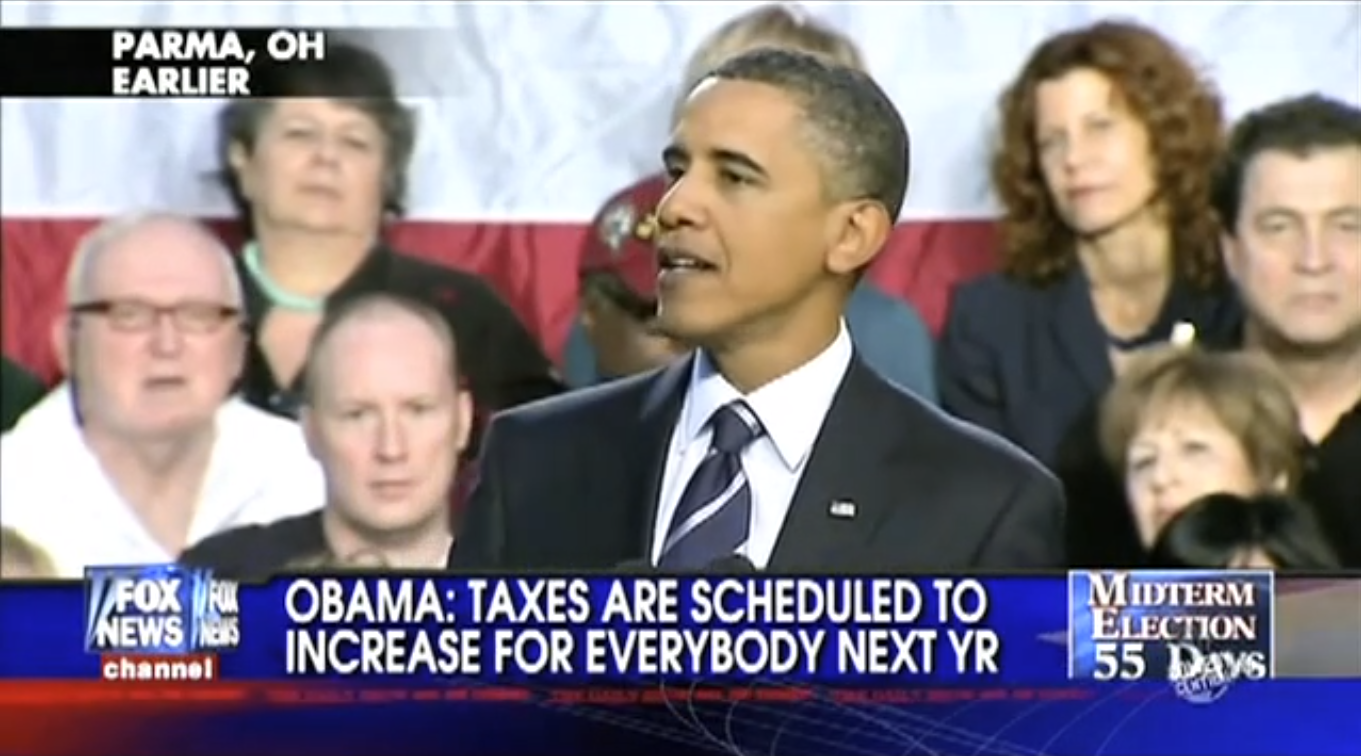
\includegraphics[width=4cm,keepaspectratio]{assets/trustworth-example-obama.png}
            \caption{Obama speech out of context.}
        }
    \end{figure}
    
\end{frame}

\section{Trustworthiness}
\begin{frame}{Trustworthiness}
    What does it mean to trust content? \pause Usually, we want \emph{novelty} and \emph{authenticity}.
    \vfill
    \pause
    \begin{block}{Authenticity}
        \pause
        \begin{itemize}
            \item Content is authentic when its origin is indisputable.\pause
            \item Can be reasonably solved with Digital Signatures.\pause
            \item Easy to check, since verifying signatures is fast.
        \end{itemize}
    \end{block}
    
    \vfill
    
    \pause
    \begin{block}{Novelty}
        \pause
        \begin{itemize}
            \item Subjective in nature, depends on the context.\pause
            \item Hard to check, requires comparing against archives.
        \end{itemize}
    \end{block}
\end{frame}

\section{Proof of Novelty}
\subsection{Overview}
\begin{frame}{Proof of Novelty}
    \begin{enumerate}
        \item[1] The owner of content $\content$ wishes to prove to us it is trustworthy.
        \item[2] A collection of similar content $\ContentSet$ exists and is secured on a blockchain with content-addressable hashes.
    \end{enumerate}
    \vfill
    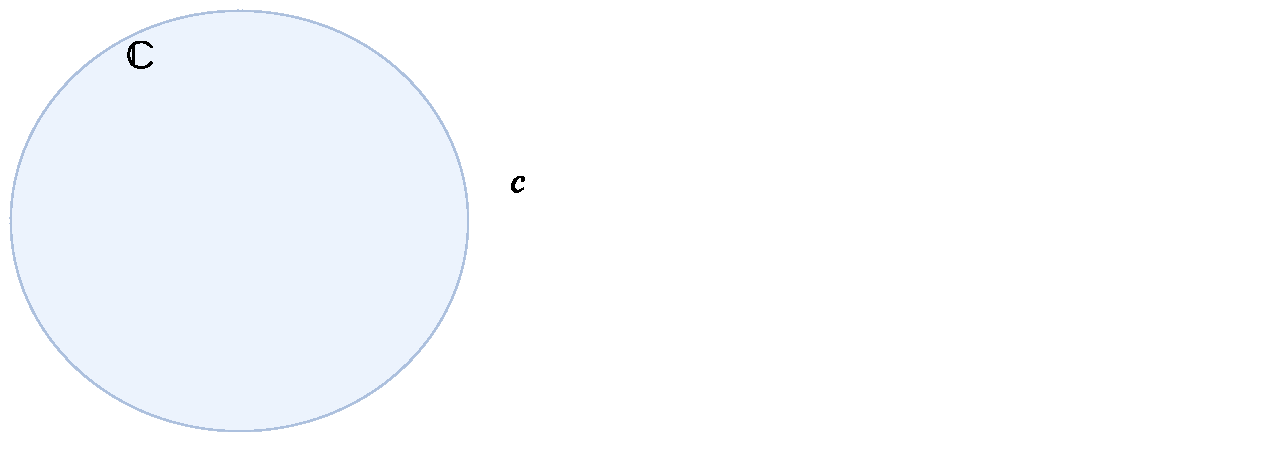
\includegraphics[width=1.0\textwidth]{assets/pon-diagram-0.pdf}
\end{frame}

\begin{frame}{Proof of Novelty}
    \begin{enumerate}
        \item[3] The owner makes a transaction on the blockchain and receives a random subset of content-hashes $\sV \subseteq \ContentSet$.
        \item[4] The owner calculates the similarity of $\content$ with the elements of $\sV$, using a predefined similarity measure.
    \end{enumerate}
    \vfill
    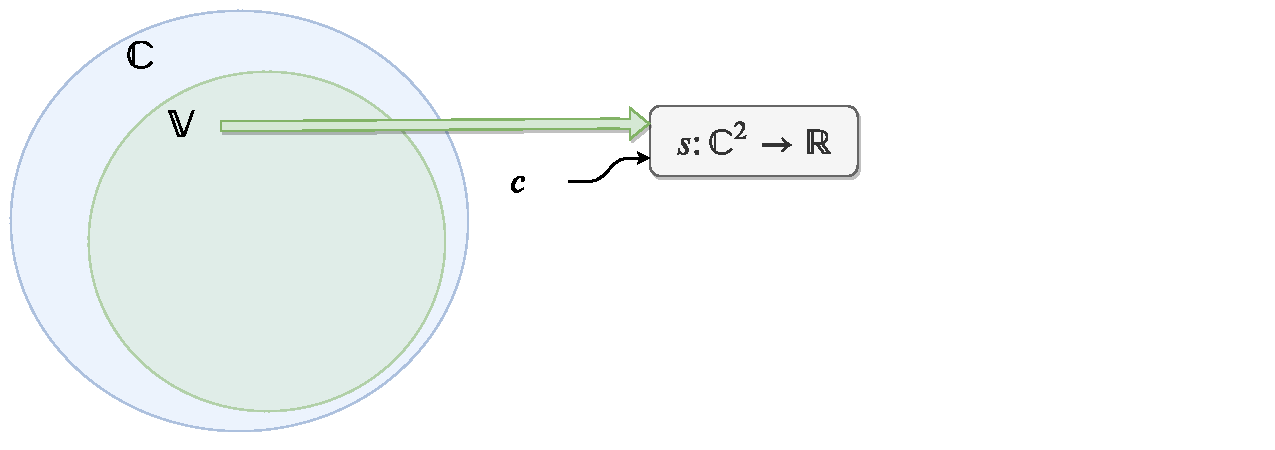
\includegraphics[width=1.0\textwidth]{assets/pon-diagram-1.pdf}
\end{frame}

\begin{frame}{Proof of Novelty}
    \begin{enumerate}
        \item[5] The blockchain chooses a random committee of peers that verify a subset of the results, $\sF \subseteq \sV$.
    \end{enumerate}
    \vfill
    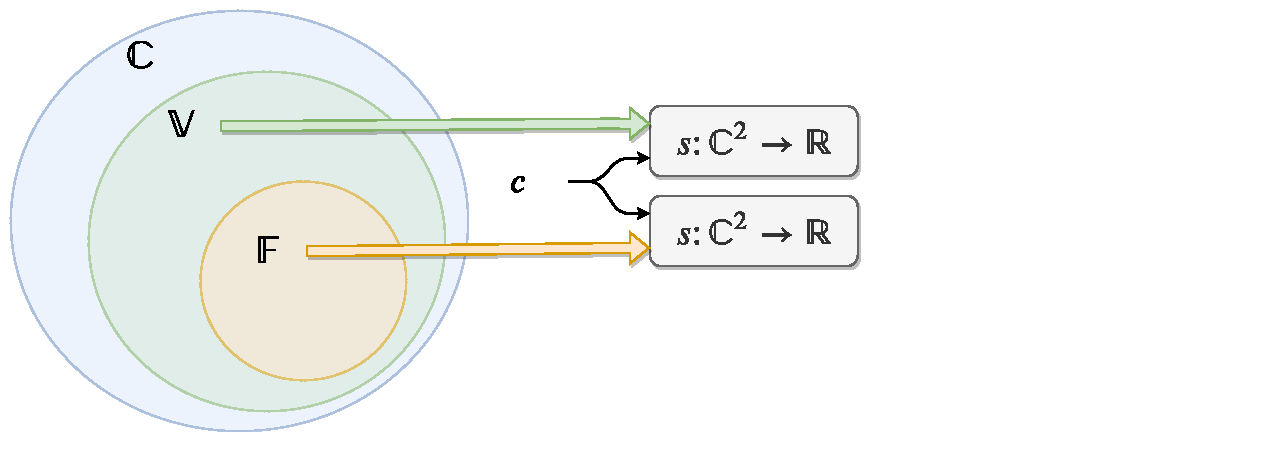
\includegraphics[width=1.0\textwidth]{assets/pon-diagram-2.pdf}
\end{frame}

\begin{frame}{Proof of Novelty}
    \begin{enumerate}
        \item[6] Consensus is reached by the committee regarding the legitimacy of the owner's calculations, and $c$ is accepted or rejected into $\ContentSet$.
    \end{enumerate}
    \vfill
    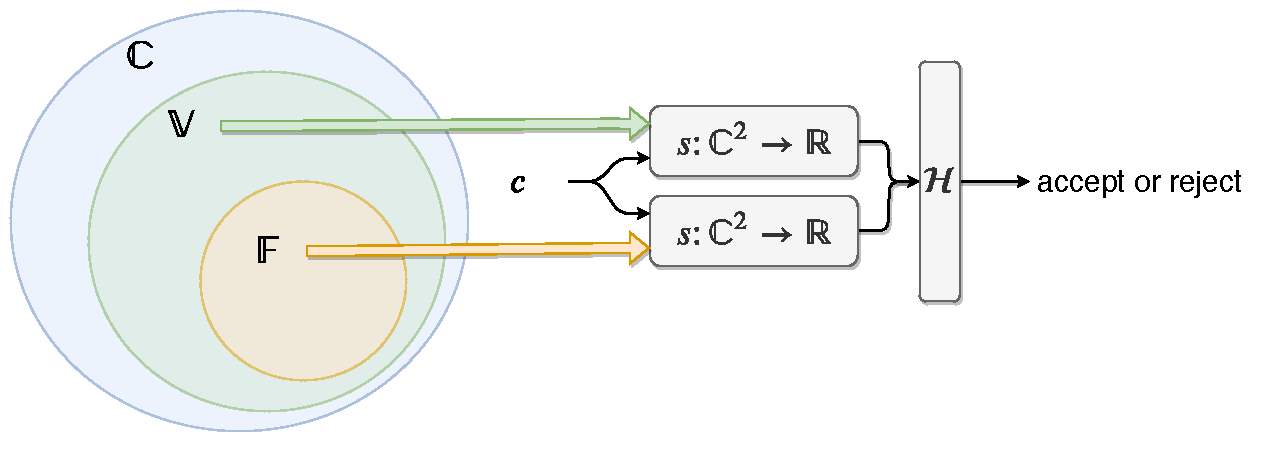
\includegraphics[width=1.0\textwidth]{assets/pon-diagram-3.pdf}
\end{frame}

\subsection{System details}
\begin{frame}{System details}
    \begin{block}{Creating $\sF$ through sortition}
        \emph{Cryptographic Sortition} can form committees without the need of interactions or exposure. Any peer holding a private key can verify and prove self-membership in the committee using a \emph{Verifiable Random Function}.
    \end{block}\pause
    \vfill
    \begin{block}{Similarity measure $s \colon \mathbb{C}^2 \rightarrow \mathbb{R}$}
        A similarity measure is any function that quantifies the degree of similarity between objects, such as a \emph{Neural Neural Network}.
    \end{block}\pause
    \vfill
    \begin{block}{Evaluating the owners submitted results}
        The committee must estimate if the similarity calculations between $c$ and elements of $\sV$ are legitimate, by observing only $\sF$.
    \end{block}
\end{frame}

\subsection{Probabilistic Guarantee of Novelty}
\begin{frame}{Probabilistic Guarantee of Novelty}
    If the owner's content is accepted, it provides a \emph{probabilistic guarantee} that their content is novel.
\end{frame}

% \begin{frame}{Proof of Novelty}
%     \begin{columns}
%         \begin{column}{0.5\textwidth}
%             \begin{enumerate}
%                 \item The owner of content $\content$ wishes to prove to us it is trustworthy.
%                 \item A collection of similar content $\ContentSet$ exists and is secured on the blockchain with content-addressable hashes.
%             \end{enumerate}
%         \end{column}
%         \begin{column}{0.5\textwidth}
%             \begin{center}
%                 \includegraphics[width=0.5\textwidth]{image1.jpg}
%             \end{center}
%         \end{column}
%     \end{columns}
% \end{frame}


\section{Take-away points}
\begin{frame}{Take-away points}
    \emph{Proof of Novelty} ...
    \begin{itemize}
        \item is a certificate issued by a decentralized and trustless system;\pause
        \item provides probabilistic guarantees of content novelty;\pause
        \item can scale by using cryptographic sortition;\pause
        \item defines similarity through similarity measures;\pause
        \item can be extended to any content type by switching the similarity measure.
    \end{itemize}
\end{frame}

\section{Open Questions and Future Work}
\begin{frame}{Open Questions and Future Work}
    \begin{itemize}
        \item Implementing and running experiments on Smart Contract blockchains such as Ethereum;\pause
        \item Applying decentralized and collaborative machine learning to progressively update a similarity function;\pause
        \item Investigating statistical hypothesis tests and guarantees
        for different content and similarity functions;\pause
        \item Properly choosing $\sV$ and $\sF$ to optimize statistical and computational performance.
    \end{itemize}
\end{frame}

% \begin{frame}{Frame Title}
% \begin{columns}
% \begin{column}{0.5\textwidth}
%   some text here some text here some text here some text here some text here
% \end{column}
% \begin{column}{0.5\textwidth}  %%<--- here
%     \begin{center}
%      \includegraphics[width=0.5\textwidth]{image1.jpg}
%      \end{center}
% \end{column}
% \end{columns}
% \end{frame}
%---------------------------------------------------------
%Changing visivility of the text
% \begin{frame}
% \frametitle{Sample frame title}
% This is a text in second frame. For the sake of showing an example.

% \begin{itemize}
%     \item<1-> Text visible on slide 1
%     \item<2-> Text visible on slide 2
%     \item<3> Text visible on slides 3
%     \item<4-> Text visible on slide 4
% \end{itemize}
% \end{frame}

%---------------------------------------------------------


%---------------------------------------------------------
% %Example of the \pause command
% \begin{frame}
% In this slide \pause

% the text will be partially visible \pause

% And finally everything will be there
% \end{frame}
%---------------------------------------------------------

% \section{Second section}

%---------------------------------------------------------
%Highlighting text
% \begin{frame}
% \frametitle{Sample frame title}

% In this slide, some important text will be
% \alert{highlighted} because it's important.
% Please, don't abuse it.

% \begin{block}{Remark}
% Sample text
% \end{block}

% \begin{alertblock}{Important theorem}
% Sample text in red box
% \end{alertblock}

% \begin{examples}
% Sample text in green box. The title of the block is ``Examples".
% \end{examples}
% \end{frame}
%---------------------------------------------------------


%---------------------------------------------------------
%Two columns
% \begin{frame}
% \frametitle{Two-column slide}

% \begin{columns}

% \column{0.5\textwidth}
% This is a text in first column.
% $$E=mc^2$$
% \begin{itemize}
% \item First item
% \item Second item
% \end{itemize}

% \column{0.5\textwidth}
% This text will be in the second column
% and on a second tought this is a nice looking
% layout in some cases.
% \end{columns}
% \end{frame}
% %---------------------------------------------------------


\end{document}